\setcounter{chapter}{2}
\chapter{Acides et Bases de Bronsted}
\section{Les acides et bases selon Brönsted}
\subsection{Exemples à connaître}
\begin{minipage}{0.7\textwidth}
Quelques exemples d'acides : \\
\trou{$\rm H_3O^+$  ; $\rm CH_3COOH$ ;  $\rm NH_4^+$ ;  $\rm H_2O$} \\
Quelques exemples de bases :\\
\trou{$\rm HO^-$ ; $\rm NH_3$ ; $\rm CH_3COO^-$  ;  $\rm H_2O$}

\subsection{Définition de Brönsted des acides et des bases}

\blocrouge{Définition}{
Un acide est une espèce capable de \trou{céder un ion Hydrogène $\rm H^+$}\\Exemple : $\rm CH_3COOH=\trou{CH_3COO^-}+H^+$\\
Une base est une espèce capable de \trou{capter un ion Hydrogène $\rm H^+$}\\Exemple : $\rm NH_3+H^+=\trou{NH_4^+}$
}

\subsection{Les couples acide/base}
Reprenons notre exemple : \\
$\rm CH_3COOH=CH_3COO^-+H^+$\\  $\rm CH_3COO^-$ est \trou{une base} puisque c'est une espèce capable de capter un ion Hydrogène. On l'appelle base conjuguée de l'acide $\rm CH_3COOH$ et on forme le couple \trou{$\rm CH_3COOH / \rm CH_3COO^-$}.\\
De façon analogue, $\rm NH_4^+$ est \trou{un acide} car capable de céder un ion Hydrogène. C'est l'acide conjugué du couple \trou{$\rm NH_4^+/NH_3$}.\\
Ecriture générale: les couples acide/base peuvent s'écrire: $\rm AH/A^-$ ou également parfois $\rm BH^+/B$

\end{minipage}
\hfill
\begin{minipage}{0.25\textwidth}

\includegraphics[scale=1]{figures/couplesAB}
\end{minipage}

\etiquette{Ex 4 p 22 questions 1 à 3}

\section{La réaction acide-base}
\subsection{Définition}

C'est une réaction ayant lieu entre \trou{l'acide} d'un couple et la base d'un \trou{autre couple}. C'est un transfert d'ion \trou{Hydrogène} de l'acide vers la base.\\
Exemple : couples $\rm HCl/Cl^-$ et $\rm H_3O^+/H_2O$\\
\trou{$\rm HCl(g)+H_2O(l)\longrightarrow Cl^-(aq)+H_3O^+(aq)$ }

\etiquette{Ex 1 p 20}
\subsection{Activité: Schéma de Lewis et Acidité}
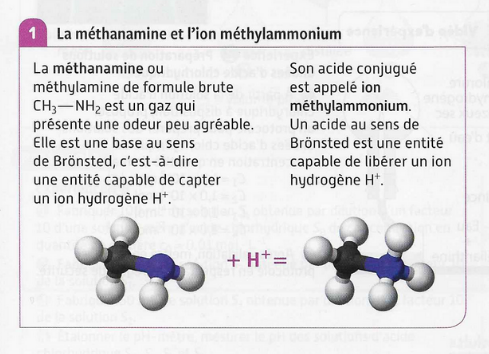
\includegraphics[scale=0.5]{figures/act_1}
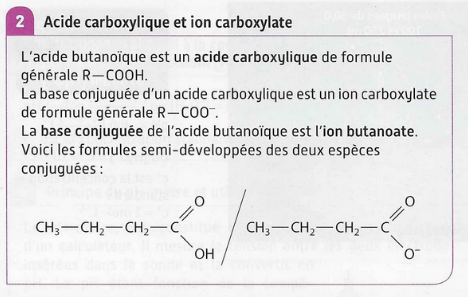
\includegraphics[scale=0.6]{figures/act_2}\\
\paragraph*{Questions}
\begin{enumerate}
	\item Écrire l'équation de la réaction acide-base entre la méthanamine et l'acide butanoïque. Nommer les produits formés.
	\item Établir la configuration électronique des différents atomes présents dans ces deux molécules.
	\item Etablir le schéma de Lewis de chacun de ces atomes.
	\item Représenter le schéma de Lewis de la méthanamine et de l'acide butanoïque.
	\item Identifier les liaisons polarisée avec l'atome d'hydrogène et représenter les éventuelles charges partielles.
	\item Entourer la liaison susceptible de se rompre dans l'acide butanoïque.
	\item Quel est l'élément libéré lors de cette rupture ? Ecrire son schéma de Lewis.
	\item Repérer dans la méthanamine le doublet non liant susceptible de venir combler la lacune électronique de l'ion hydrogène.
	\item Conclusion : En vous appuyant sur le schéma de Lewis justifier le transfert d'ion hydrogène H+ entre l'acide butanoïque et la méthanamine.
\end{enumerate}


\section{Quelques couples acide-base}
\subsection{Les couples des acides carboxyliques}
Un acide carboxylique de formule $RCO_2H$ cède un ion hydrogène $H^+$ pour former un ion carboxylate $RCO_2^-$\\

Ecrire les formules de Lewis de l'acide butanoïque et de l'ion butanoate.
 
\subsection{Les couples de l'eau}
L'eau $H_2O$ appartient à deux couples :
\begin{itemize}
\item Le couple $\trou{H_3O^+}/H_2O$ où elle joue le rôle de la base
\item Le couple $H_2O/\trou{HO^-}$ où elle joue le rôle de l'acide
\end{itemize}
L'eau se comporte soit comme un acide soit comme une base. On dit que l'eau est une espèce \trou{amphotère ou un ampholyte.}
\subsection{Les couples de l'acide carbonique}

L'acide carbonique $H_2CO_3$ est un acide instable qui se forme lors de la dissolution du dioxyde de carbone dans l'eau selon l'équation :
$$CO_{2(g)} + H_2O_{(l)} \leftrightharpoons H_2CO_{3(aq)}$$

La base conjuguée de l'acide carbonique est l'ion hydrogénocarbonate  de formule\trou{   $HCO_3^-$} 

L'ion hydrogénocarbone est un acide, il peut libérer un ion $H^+$ et former un ion carbonate de formule \trou{$CO_3^{2-}$}.

\etiquette{Résumé}

$ H_2CO_3(aq) =  \trou{HCO_3^-} + H^+$\\
$\trou{HCO_3^- }=  CO_3^{2-} +\trou{ H^+}$\\

L'espèce $\trou{HCO_3^-}$ étant à la fois base et acide, c'est, tout comme l'eau, une espèce \trou{amphotère}.\\


\etiquette{Astuce importante} Lorsqu'un exercice parle de dioxyde de carbone dissous, pensez à l'acide carbonique $H_2CO_3$ que l'on écrira très souvent  $CO_2(aq),H_2O(l)$.

\subsection{Les couples des amines}
Les amines sont des molécules azotées, obtenues par remplacement de 1, 2 ou 3 atomes d'hydrogène par 1, 2 ou 3 groupes alkyles.\\
Grâce au\trou{ doublet non liant} porté par l'atome d'azote, les amines sont des espèces capables de capter un ion $H^+$, les amines sont donc des\trou{ bases}.\\


Ecrire les formules de Lewis d'une amine en notant $R_1$, $R_2$ et $R_3$ les groupes liés à l'azote et de l'ion ammonium associé.


\section{Mesure de l'acidité d'une solution}
\subsection{pH}

\blocrouge{Définition}{Le pH d'une solution est un nombre sans unité qui indique l'acidité d'une solution. L'acidité d'une solution est d'autant plus \trou{grande} que le pH est \trou{petit}. Plus la concentration en \trou{ion hydrogène} est grande, plus le pH est petit.

$$\trou{pH = -\log \left(\frac{[H_3O^+]}{c_0}\right)}$$ \trou{avec $c_0 = 1$ mol/L}

A partir de la valeur du pH de la solution, on peut déterminer la concentration des ions hydrogène: $$\trou{[H_3O^+]=10^{-pH}}$$

}

\paragraph*{Remarque} 
\begin{itemize}
 	\item La formule permettant de calculer le pH n'est valable que pour une concentration inférieure à \trou{0,05 mol/L}.

\end{itemize}
\subsection{Exemples et calculs}

\begin{itemize}
\item Le pH d'une solution $S_1$ de concentration en ions oxonium égale à $1,0\cdot 10^{-3}$ mol/L vaut: \trou{$pH = - \log(\frac{[H_3O^+]}{c_0})=-\log(\frac{1,0.10^{-3}\: mol/L}{1\:mol/L}=3,0)$}
\item Le pH d'un soda (considéré comme une solution aqueuse) vaut 2,5. Vérifier que la concentration des ions $H_3O^+$ vaut 3,2 mmol/L.
\end{itemize}

\blocrouge{Exercices à faire} {
\begin{itemize}
	\item 14,15,16 p 24-25 
	\item  20 + prépa ECE p27
\end{itemize}
}